% Source: fixed PDF source-relative page 1 (printed page 306), Q15.
% Prism edges and fine route trace follow the source image; route endpoints are schematic where source strokes meet thin edges.
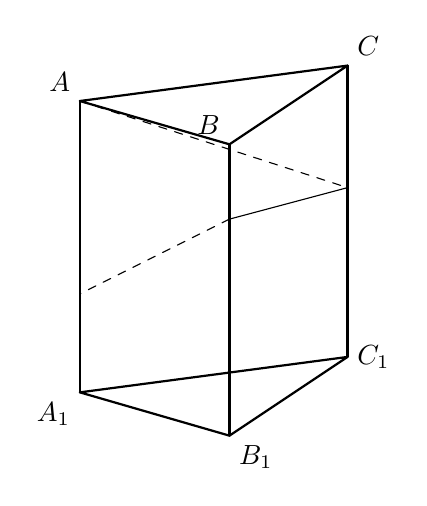
\begin{tikzpicture}[line cap=round,line join=round]
  \coordinate (A) at (0,3.7);
  \coordinate (B) at (1.9,3.15);
  \coordinate (C) at (3.4,4.15);
  \coordinate (A1) at (0,0);
  \coordinate (B1) at (1.9,-0.55);
  \coordinate (C1) at (3.4,0.45);
  \coordinate (Mab) at (1.9,2.2); % point on BB1
  \coordinate (Mc) at (3.4,2.6); % point on CC1
  \coordinate (Ma) at (0,1.25);  % point on AA1
  % Triangular prism edges
  \draw[thick] (A)--(B)--(C)--cycle;
  \draw[thick] (A)--(A1) (B)--(B1) (C)--(C1);
  \draw[thick] (A1)--(B1)--(C1)--cycle;
  % The source depicts a fine, winding trace over the lateral faces.
  % Hidden portions of the trace are dashed as in the source drawing.
  \draw[thin,dashed] (A)--(Mc);
  \draw[thin] (Mc)--(Mab);
  \draw[thin,dashed] (Mab)--(Ma);
  \draw[thin,dashed] (Ma)--(A1);
  \node[above left] at (A) {$A$};
  \node[below left] at (A1) {$A_1$};
  \node[above left] at (B) {$B$};
  \node[below right] at (B1) {$B_1$};
  \node[above right] at (C) {$C$};
  \node[right] at (C1) {$C_1$};
\end{tikzpicture}
